%*******10********20********30********40********50********60********70********80

% For all chapters, use the newdefined chap{} instead of chapter{}
% This will make the text at the top-left of the page be the same as the chapter

\chap{Generative Adversarial Network}
\section{Introduction}

The basic building block of this work is generative adversarial network. After the first published by Ian \textit{et al.} \cite{Original-GAN} , there have lot of recent advancements in generative adversarial networks. It has now become one of the most studied generative model. A lot of variations and different architectures have been developed after the first paper was published. In this chapter, we explain GAN from the very basics.

\section{Generative Model}
Generative adversarial networks works on the principle of maximum likelihood.
%[https://arxiv.org/pdf/1701.00160.pdf].
It means, when given a dataset, the model tries to provide probability distribution of the sample data, parametrized by $\theta$. %As this work is focused on computer vision,so the key relationship between images and statistics is that we can interpret images as samples from a high-dimensional probability distribution.
\par
The generative models based on maximum likelihood can be based divided into explicit and implicit density model. Below figure differentiates different models based on the maximum likelihood principal.
%
\begin{figure}[h]
    
    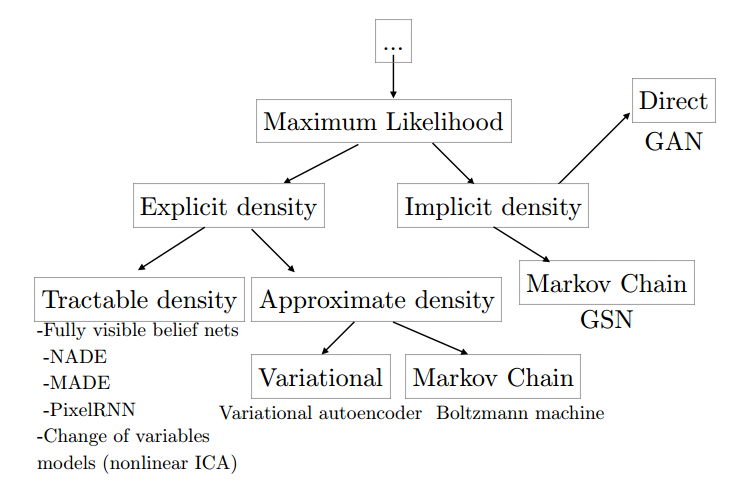
\includegraphics[scale=.6, angle=0]{Files/taxanomy.png}
    \caption[The panther]{Taxonomy of Generative Model\cite{GanTut}}
    \label{fig: jordan}
\end{figure}

In explicit model, also known as prescribed probabilistic model, we explicitly define the distribution of random variable and specify the log likelihood function.
In implicit model we don't need to define the density function\cite{1}. The model learn the function from the data and generate sample in a single step.
%SJ:Grammatical error

\section{The GAN  Concept}
Generative Adversarial network works by inter playing two deep artificial neural networks, a generator(G) and a discriminator(D). Both of these networks play a min max game, where generator tries to produce a fake image and discriminator tries to identify whether it is a fake or a real image, as illustrated in Figure 3.2. In the below figure the generator is provided a with random noise to produce a fake data sample , whereas the discriminator is given both the real and fake image and it tries to classifies these data sample.
%SJ:is figure number correct
\begin{figure}[t]

  \centering
    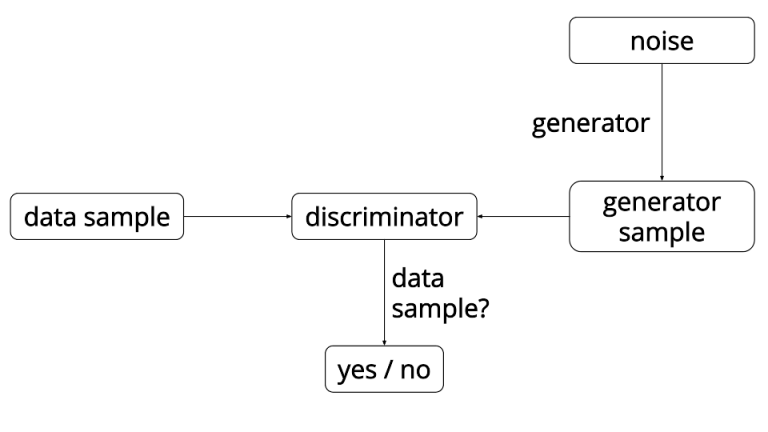
\includegraphics[scale=.4, angle=0]{Files/gan-overview.png}
    \caption[GAN overview]{ GAN overview\cite{Gan-overview}}
    \label{fig: GAN-Overview}
\end{figure}
\newpage
\subsection{Mathematical Definition}
Mathematically, let x,  $\theta_{G}$  and $\theta_{D}$ be data variables, optimal hyper-parameters of the generator and discriminator model.
Given a latent variable z, drawn from a Gaussian distribution, the generator transforms this variable to a sample from the data. And the discriminator tries to estimate whether x is from the data space $p_{data}$. The final objective function F becomes
$$ \substack{min\\ G} \substack{max\\ D} F (\theta_{G}, \theta_{D}) = E_{x\sim p_{data}} [log (D (x; \theta_{D}))] + E_{z\sim N(0,I)}\log (1- D(G (z; \theta_{G}) ; \theta_{D}))$$
\subsection{Real World Example}
To understand GAN better, lets take a real world analogy. Suppose G is a counterfeit artist, who produces fake money and D is an undercover agent from FBI, who is acting as a buyer. The task of D is to differentiate the money. To master this skill, G produces a fake currency batch and sells it to D. If D identifies the batch then G updates its skill based on feedback from D. %SJ:feedback from G or D?
In this way, both go back and forth, till G has learnt the art of producing fake money.
\section{Algorithm}
In this section we provide a basic algorithm for GAN. Basically for each iteration, we sample k noises and generate sample using generator.Now we feed this mini-batch of generated data sample with real data to discriminator and update it using stochastic gradient. Since we cannot directly compute the loss for generator, so we use discriminator gradient but in opposite direction.The reason for going opposite is because we are training discriminator to accurately predict real sample whereas generator we re training it to produce synthetic data sample. The below figure gives the actual algorithm.
\begin{figure}[!htb]

  \centering
    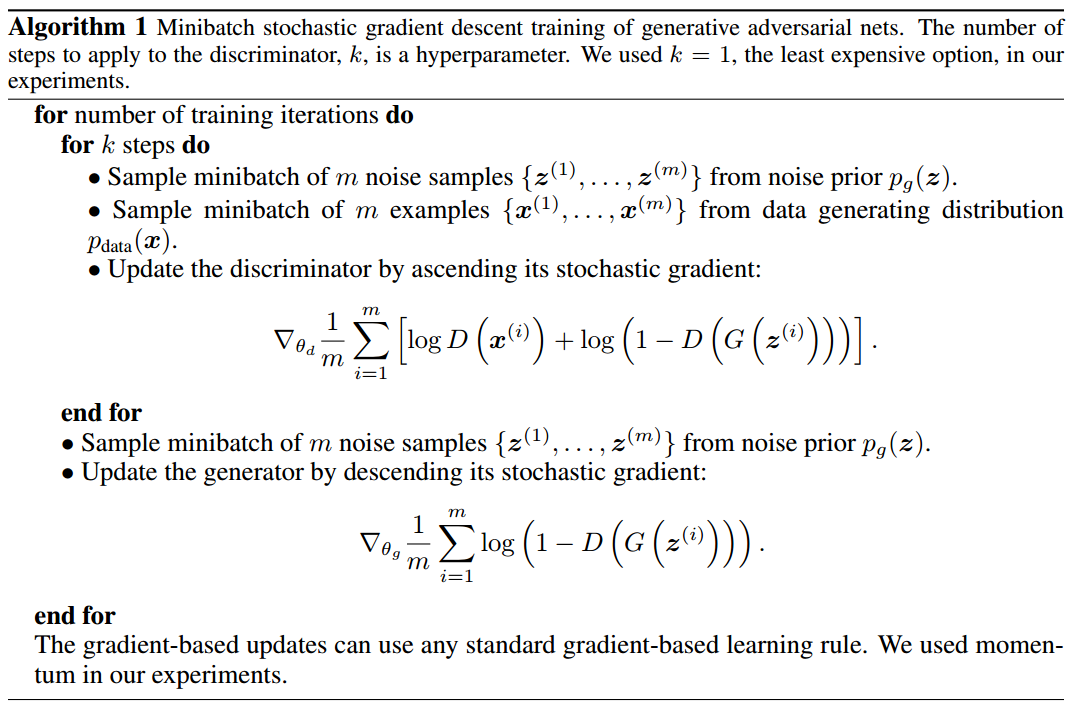
\includegraphics[scale=.4, angle=0]{Files/Algorithm.png}
    \caption[Vanilla GAN Algorithm]{ GAN Algorithm\cite{Gan-overview}}
    \label{fig: GAN Algorithm}
\end{figure}

\section{Analysis}

We can analyse the discriminator to see why GAN is effective. The basic idea is when we take derivative of the equation in section 3.3.1 with respect to discriminator function, then the final equation is the ratio of data distribution of .
%SJ:doesnt feel correct
$$ D(x) =\frac{p_{data}}{p_{data} + p_{model}}$$

So, basically we are learning the ratio data density and the model density. In the below figure we can visualize the approach. The green  line is the$p_{model}$ which is generated by our generator G, the black line depicts our actual data distribution $p_{data}$ and the blue line is of discriminator differentiating real and generated data. The horizontal line z, below the graph is domain of the latent variable drawn from uniform gaussian %SJ:capital G?
distribution and x is the data domain. The arrow indicates G(z). 
\begin{figure}
  \centering
    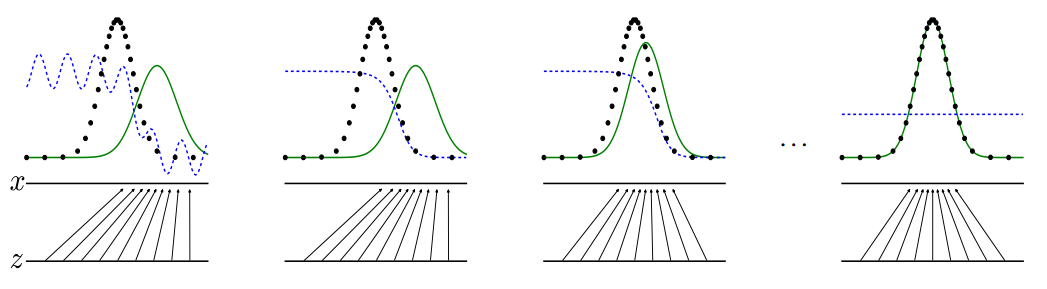
\includegraphics[scale=.4, angle=0]{Files/GAN-Visualize.png}
    \caption[GAN Algorithm Visualization]{ GAN Graphical Explanation\cite{Gan-overview}}
    \label{fig: GAN Graphical Explanation}
\end{figure}

\section{Images as Data}

As explained above we can use GAN to model the data. Now to use images as data, we have to look at the images from statistical point of view.  Images can be defined using probability density function. The probability density function gives us the likelihood of random variable, given the distribution. So if we have a large dataset of images then, we can visualize these images as PDFs in higher dimension space.
%SJ:and or then in earlier sentence?
The complexity of the distribution depends upon the number of images. Thus, our generator tries to find the true PDF from the real world data and generate images from it.
%SJ:of or from?